% Preamble template for Tufte-style lecture notes.
% Do not compile this file directly; compile the main notes file instead.
\documentclass{tufte-handout}

\usepackage{ntheorem}
\usepackage{graphicx}
\usepackage{amsmath}
\usepackage{amssymb}
\usepackage{hyperref}
\usepackage{epigraph}
\usepackage{booktabs}
\theoremstyle{break}
% \usepackage[
% bibencoding=utf8,% .bib file encoding
% maxbibnames=3, % otherwise et al
% minbibnames=1, % otherwise et al
% backend=biber,%
% sortlocale=en_US,%
% style=apa,% or authoryear
% % apabackref=false, % backreferences
% natbib=true,% for citet/citep, but this is for backward compatibility
% uniquename=false,%
% url=true,%
% sortcites=false,
% doi=true,%
% eprint=true%
% ]{biblatex}
% \addbibresource{lecture_note_bib.bib}

\hypersetup{
  colorlinks,
  urlcolor = blue,
  pdfauthor={Paul Goldsmith-Pinkham}
  pdfkeywords={econometrics}
  pdftitle={Lecture Notes for Applied Empirical Methods}
  pdfpagemode=UseNone
}
\newtheorem{ruleN}{Rule}
\newtheorem{thmN}{Theorem}
\newtheorem{assN}{Assumption}
\newtheorem{defN}{Definition}
\newtheorem{exmp}{Example}
\newtheorem{cmt}{Comment}
\newtheorem{proof}{Proof}

\newcommand{\continuation}{??}
\newtheorem*{excont}{Example \continuation}
\newenvironment{continueexample}[1]
 {\renewcommand{\continuation}{\ref{#1}}\excont[continued]}
 {\endexcont}
\newcommand{\bY}{\mathbf{Y}}
\newcommand{\bX}{\mathbf{X}}
\newcommand{\bD}{\mathbf{D}}
\newcommand{\E}{\mathbb{E}}

\newcommand\independent{\protect\mathpalette{\protect\independenT}{\perp}}
\def\independenT#1#2{\mathrel{\rlap{$#1#2$}\mkern2mu{#1#2}}}
\DeclareMathOperator{\Supp}{Supp}

\usepackage{cleveref}
\crefname{appsec}{appendix}{appendices}
\crefname{appsubsec}{appendix}{appendices}
\crefname{assumption}{assumption}{assumptions}
\crefname{equation}{equation}{equations}
\crefname{exmp}{example}{examples}
\crefname{assN}{assumption}{assumptions}
\crefname{cmt}{comment}{comments}
\crefname{defN}{definition}{definitions}

\usepackage[nolist]{acronym}
\begin{acronym}
  \acro{CI}{confidence interval}%
  \acro{OLS}{ordinary least squares}%
  \acro{CLT}{central limit theorem}%
  \acro{IV}{instrumental variables}%
  \acro{ATE}{average treatment effect}%
  \acro{RCT}{randomized control trial}%
  \acro{SUTVA}{stable unit treatment value assignment}
  \acro{VAM}{value-added model}%
  \acro{LAN}{locally asymptotically normal}%
  \acro{DiD}{difference-in-differences}%
  \acro{OVB}{omitted variables bias}
  \acro{FWL}{Frisch-Waugh-Lovell}
  \acro{DAG}{directed acyclic graph}
  \acro{PO}{potential outcomes}
\end{acronym}

\def\inprobHIGH{\,{\buildrel p \over \rightarrow}\,} 
\def\inprob{\,{\inprobHIGH}\,} 
\def\indistHIGH{\,{\buildrel d \over \rightarrow}\,} 
\def\indist{\,{\indistHIGH}\,}

\usepackage[many]{tcolorbox} 
\definecolor{main}{HTML}{3F6EA7}      % primary accent
\definecolor{sub}{HTML}{F2F7FD}       % cool background
\definecolor{sub2}{HTML}{FFF5E8}      % warm background
\definecolor{mainline}{HTML}{D3DFEE}  % soft frame for information boxes
\definecolor{warn}{HTML}{C7771B}      % accent for caution boxes
\definecolor{warnline}{HTML}{EAD9C0}  % soft frame for caution boxes

\tcbset{
    enhanced,
    breakable,
    colback = white,
    boxrule = 0.5pt,
    arc = 2pt,
    left = 9pt,
    right = 9pt,
    top = 7pt,
    bottom = 7pt,
    before skip = 0.3cm,
    after skip = 0.45cm
}                           % setting global options for tcolorbox

\newtcolorbox{boxD}{
    colback = sub,
    colframe = mainline,
    borderline west = {2.2pt}{0pt}{main},
    borderline north = {0.6pt}{0pt}{main!25},
    borderline south = {0.6pt}{0pt}{main!15}
}


\newtcolorbox{boxF}{
    colback = sub2,
    colframe = warnline,
    borderline west = {2.2pt}{0pt}{warn},
    borderline north = {0.6pt}{0pt}{warn!25},
    borderline south = {0.6pt}{0pt}{warn!15}
}

\usepackage{colortbl}


\usepackage{tikz}
\usepackage{verbatim}
\usetikzlibrary{positioning}
\usetikzlibrary{snakes}
\usetikzlibrary{calc}
\usetikzlibrary{arrows}
\usetikzlibrary{decorations.markings}
\usetikzlibrary{shapes.misc}
\usetikzlibrary{matrix,shapes,arrows,fit,tikzmark}




\title{S181M116 Derivatives and Alternative Investments: Lecture 1}
\author{Swapnil Singh}
\date{}

\hypersetup{
  pdftitle={S181M116 Derivatives and Alternative Investments: Lecture 1},
  pdfauthor={Swapnil Singh},
  pdfkeywords={derivatives, futures, forwards, options, clearing, margin, risk management}
}

\setlength{\headheight}{26pt}
\graphicspath{{images/lecture-1/}}

\newcommand{\St}{S_T}
\newcommand{\Fzero}{F_0}
\newcommand{\Ft}{F_t}
\newcommand{\K}{K}
\newcommand{\pnl}{\mathrm{P\&L}}
\newcommand{\PV}{\mathrm{PV}}

\begin{document}
\maketitle

\begin{abstract}
This lecture introduces the basic language and market architecture of derivatives.
We study forwards, futures, options, exchanges, OTC markets, clearing houses,
margin accounts, and the first no-arbitrage arguments. We also use major
derivatives mishaps to establish a risk-management discipline that will remain
important throughout the course.
\end{abstract}

\begin{boxD}
\textbf{Reading.} Hull, Chapters 1, 2, and selected lessons from Chapter 37.
The goal is not to memorize institutional detail. The goal is to understand how
contract design, clearing, collateral, and no-arbitrage logic determine who bears
which risks.
\end{boxD}

\section{What Is a Derivative?}

A \emph{derivative} is a financial contract whose value depends on an underlying
variable. The underlying may be a traded asset price, such as a stock price,
bond price, commodity price, exchange rate, or stock index. It may also be a
rate, spread, credit event, weather variable, or other observable quantity.

\begin{defN}[Derivative]
A derivative contract specifies cash flows at one or more future dates as a
function of one or more underlying variables. If $X_T$ denotes the relevant
underlying variable at date $T$, the derivative payoff can often be written as
\[
    g(X_T),
\]
where $g(\cdot)$ is the payoff function.
\end{defN}

This definition is deliberately broad. A forward contract has payoff linear in
the future asset price. A call option has a nonlinear payoff. A swap is a
portfolio of future exchanges of cash flows. A credit default swap pays when a
credit event occurs. The common element is that the contract derives its value
from something else.

\begin{marginfigure}
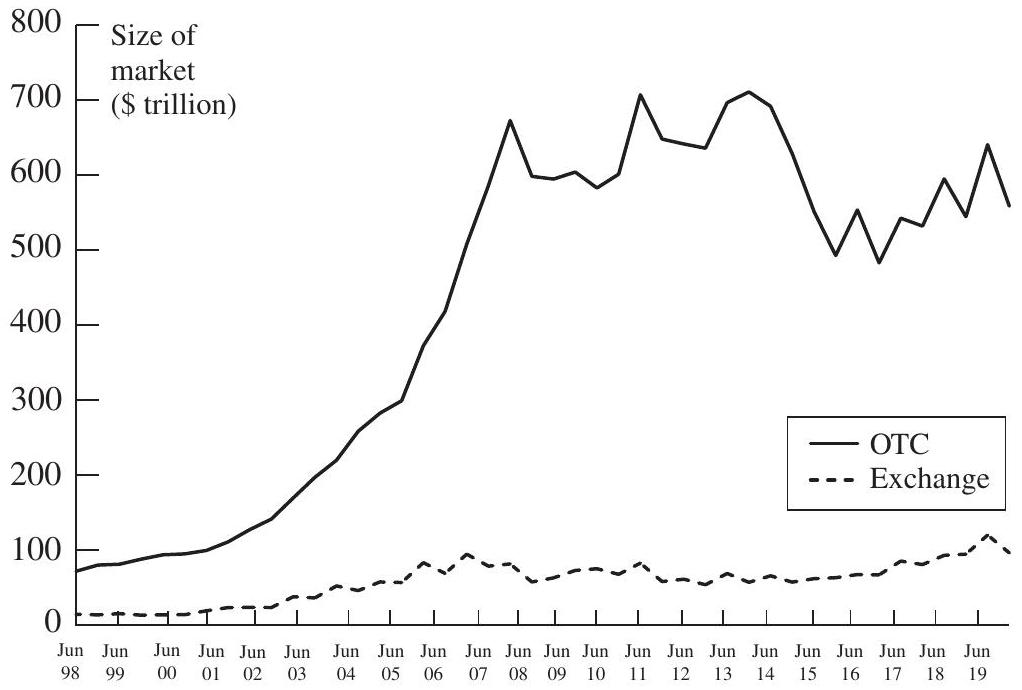
\includegraphics[width=\linewidth]{ead832f5-1069-4974-84bd-4a1adcf0b304-027_690_1022_1578_365.jpg}
\caption{Derivative markets are large relative to underlying cash markets. The
notional amount is not the same as market value, but it measures scale and
interconnectedness.}
\end{marginfigure}

There are three reasons derivatives matter.
\begin{enumerate}
    \item \textbf{Risk transfer.} A firm can transfer commodity, interest-rate,
    foreign-exchange, or equity risk to another party.
    \item \textbf{Price discovery and leverage.} Derivatives allow market
    participants to take positions with limited initial cash outlay.
    \item \textbf{Replicating logic.} Derivative prices are tightly connected
    to prices of underlying assets, interest rates, and other derivatives.
\end{enumerate}

\begin{boxF}
\textbf{Important distinction.} A derivative can reduce risk for one party and
increase risk for another. The contract itself is not ``safe'' or ``dangerous.''
Its effect depends on the position, leverage, collateral, liquidity, and the
institution's ability to manage the exposure.
\end{boxF}

\section{Payoff, Profit, and Value}

We will use three related but different concepts throughout the course.
\begin{description}
    \item[Payoff] The cash flow at maturity, usually written as a function of
    the terminal underlying price.
    \item[Profit] The payoff net of the initial cost and any financing cost.
    \item[Value] The market value of the contract today, before maturity.
\end{description}

For a contract with payoff $g(S_T)$ at maturity $T$, the value today is not
generally $g(S_0)$. Valuation discounts, risk-adjusts, or replicates the future
payoff. The central intellectual move in derivatives is to ask:

\begin{quote}
Can this future payoff be replicated by trading other assets?
\end{quote}

If yes, the derivative's price is pinned down by no-arbitrage. If not exactly,
pricing requires a model, a convention, or a market quote.

\section{Market Architecture}

\subsection{Exchange-Traded Markets}

An exchange-traded derivative is standardized by an exchange. The exchange
specifies the underlying asset, contract size, maturity cycle, delivery or cash
settlement rules, tick size, and trading procedures. Standardization makes
anonymous trading and liquidity easier.

The clearing house is central. Once a trade is matched, the clearing house
becomes the buyer to every seller and the seller to every buyer. This process is
called \emph{novation}. It replaces bilateral counterparty exposure with exposure
to the clearing house.

\begin{boxD}
\textbf{Exchange-traded derivative.} The trader cares less about the identity of
the counterparty because the clearing house stands between the two sides. Credit
risk is controlled through margin, daily settlement, default funds, and member
capital.
\end{boxD}

\subsection{Over-the-Counter Markets}

An over-the-counter (OTC) derivative is negotiated privately. OTC contracts are
more flexible than exchange-traded contracts: maturity, notional, payoff, and
collateral terms can be customized. The cost of customization is weaker
standardization and potentially greater counterparty, liquidity, and valuation
risk.

Modern OTC markets often use central counterparties for standardized trades, but
many contracts remain bilateral. Bilateral OTC trading is governed by legal
agreements that define close-out netting, collateral, default events, and
valuation procedures.

\begin{marginfigure}
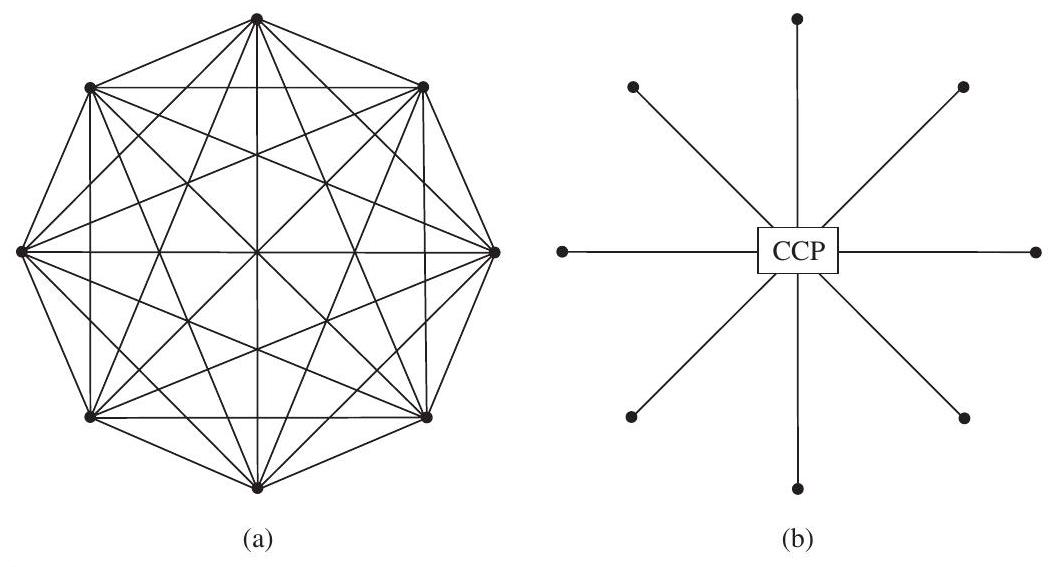
\includegraphics[width=\linewidth]{ead832f5-1069-4974-84bd-4a1adcf0b304-057_567_1059_410_359.jpg}
\caption{Bilateral OTC links create a network of counterparty exposures. A CCP
changes the network but concentrates risk management in one institution.}
\end{marginfigure}

\subsection{Notional Amount Versus Market Value}

The \emph{notional principal} is the reference amount used to compute payments.
It is not usually the amount at risk. For example, in a forward contract to
exchange GBP 1 million for dollars, the notional is GBP 1 million. The market
value may be only a small fraction of that amount because only the difference
between the contracted exchange rate and the current forward rate is at stake.

Nevertheless, notional matters because it measures scale. A small percentage move
on a large notional can produce a large gain or loss.

\section{Forward Contracts}

\subsection{Definition and Payoffs}

A forward contract is an agreement to buy or sell an asset at a specified future
date $T$ for a specified delivery price $\K$. The party that agrees to buy has a
\emph{long forward position}. The party that agrees to sell has a \emph{short
forward position}.

\begin{defN}[Forward payoff]
For one unit of the underlying asset, the payoff at maturity is
\[
    \text{Long forward payoff} = \St-\K,
\]
and
\[
    \text{Short forward payoff} = \K-\St.
\]
\end{defN}

\begin{figure}
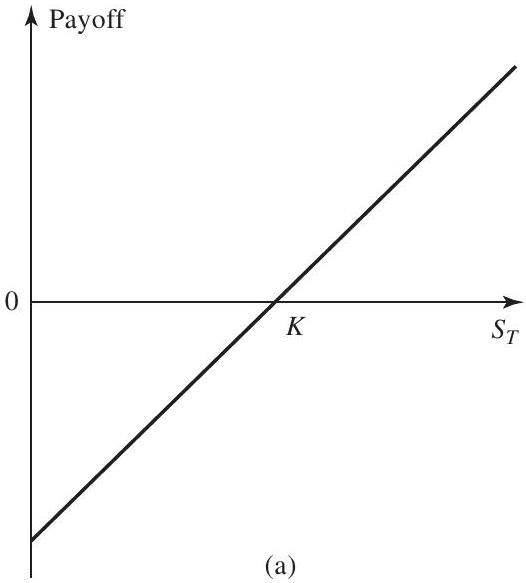
\includegraphics[width=0.48\linewidth]{ead832f5-1069-4974-84bd-4a1adcf0b304-030_583_526_380_457.jpg}
\hfill
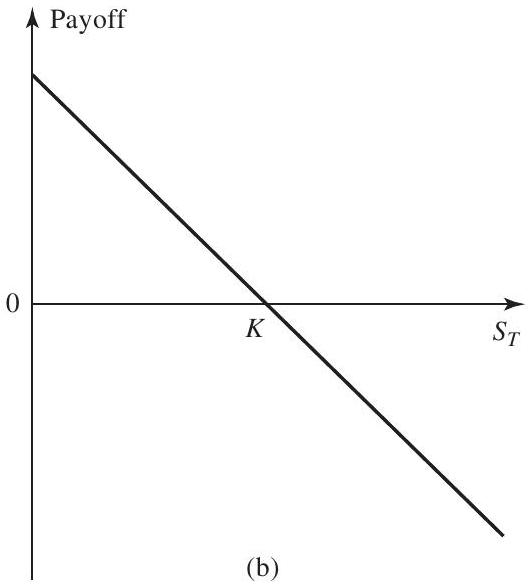
\includegraphics[width=0.48\linewidth]{ead832f5-1069-4974-84bd-4a1adcf0b304-030_585_528_378_1111.jpg}
\caption{Forward payoffs. A long forward gains when the terminal spot price is
above the delivery price. A short forward gains when it is below the delivery
price.}
\end{figure}

The payoff is linear. This linearity is what makes forwards useful for hedging.
If a firm knows it must buy an asset in the future, a long forward locks in the
purchase price. If a firm knows it must sell an asset in the future, a short
forward locks in the sale price.

\begin{exmp}[Foreign-exchange hedge]
A U.S. firm must pay GBP 1 million in six months. The six-month forward quote is
USD 1.2230 per GBP. By entering a long forward on GBP, the firm commits to pay
USD 1.223 million for GBP 1 million at maturity.

If the future spot exchange rate is 1.3000, the forward payoff is
\[
    (1.3000-1.2230)\times 1{,}000{,}000 = \$77{,}000.
\]
If the future spot exchange rate is 1.2000, the payoff is
\[
    (1.2000-1.2230)\times 1{,}000{,}000 = -\$23{,}000.
\]
The hedge removes uncertainty about the dollar cost, but it also removes the
benefit of a favorable exchange-rate movement.
\end{exmp}

\subsection{Forward Price Versus Delivery Price}

The \emph{delivery price} $\K$ is the price written into an existing contract.
The \emph{forward price} $\Fzero$ is the delivery price that would make a newly
negotiated forward contract have zero value today.

At initiation, a standard forward usually has zero value:
\[
    f_0 = 0.
\]
That does not mean the contract is worthless economically. It means neither side
pays an upfront premium because the agreed delivery price is set fairly relative
to current market conditions.

\subsection{A First No-Arbitrage Derivation}

Consider a non-dividend-paying stock with current price $S_0$. Suppose the
risk-free continuously compounded interest rate is $r$ and maturity is $T$. We
derive the no-arbitrage forward price.

\begin{thmN}[Forward price for a non-income asset]
For an asset with no income and no storage cost, under frictionless markets,
\[
    \Fzero = S_0 e^{rT}.
\]
\end{thmN}

\begin{proof}
First suppose the quoted forward price is too high:
\[
    \Fzero > S_0 e^{rT}.
\]
Construct the following strategy at time 0:
\begin{enumerate}
    \item Borrow $S_0$ at the risk-free rate.
    \item Buy one share of the stock.
    \item Enter a short forward contract to sell the stock for $\Fzero$ at $T$.
\end{enumerate}
At time $T$, deliver the stock into the forward contract and receive $\Fzero$.
Repay the loan, which has grown to $S_0e^{rT}$. The terminal profit is
\[
    \Fzero-S_0e^{rT} > 0.
\]
There was no initial net investment. This is an arbitrage.

Now suppose the quoted forward price is too low:
\[
    \Fzero < S_0 e^{rT}.
\]
If short selling is possible, construct the reverse strategy:
\begin{enumerate}
    \item Short sell one share and receive $S_0$.
    \item Invest $S_0$ at the risk-free rate.
    \item Enter a long forward contract to buy the stock for $\Fzero$ at $T$.
\end{enumerate}
At time $T$, the investment is worth $S_0e^{rT}$. Use $\Fzero$ to buy the stock
under the forward contract and return it to close the short sale. The terminal
profit is
\[
    S_0e^{rT}-\Fzero > 0.
\]
Again, this is an arbitrage. Therefore the only no-arbitrage price is
$\Fzero=S_0e^{rT}$.
\end{proof}

\begin{boxF}
\textbf{Intuition.} A forward contract postpones payment for the asset. If the
asset pays no income, the forward price should equal today's spot price grown at
the financing rate. Otherwise, traders can choose between ``buy now and finance''
and ``agree to buy later'' to lock in a profit.
\end{boxF}

\section{Futures Contracts}

\subsection{How Futures Differ from Forwards}

A futures contract is also an agreement to buy or sell an asset at a future date
for a price agreed today. The key differences are institutional:
\begin{itemize}
    \item Futures are exchange-traded and standardized.
    \item Futures are marked to market daily.
    \item Traders post initial margin and must maintain a minimum margin balance.
    \item Most futures positions are closed out before delivery.
    \item The clearing house becomes the counterparty to both sides.
\end{itemize}

\begin{table}
\centering
\begin{tabular}{p{0.28\linewidth}p{0.28\linewidth}p{0.28\linewidth}}
\toprule
Feature & Forward & Futures \\
\midrule
Trading venue & OTC & Exchange \\
Terms & Customized & Standardized \\
Counterparty risk & Bilateral or CCP & Clearing house \\
Settlement & Usually at maturity & Daily mark-to-market \\
Initial cash flow & Usually none & Margin deposit \\
Closing position & Negotiated offset & Exchange offset is easy \\
\bottomrule
\end{tabular}
\caption{Forward and futures contracts have similar economic exposure but very
different market plumbing.}
\end{table}

\subsection{Convergence to the Spot Price}

As the delivery period approaches, the futures price must converge to the spot
price of the deliverable asset, after adjusting for any contract-specific
delivery options or quality differences.

\begin{marginfigure}
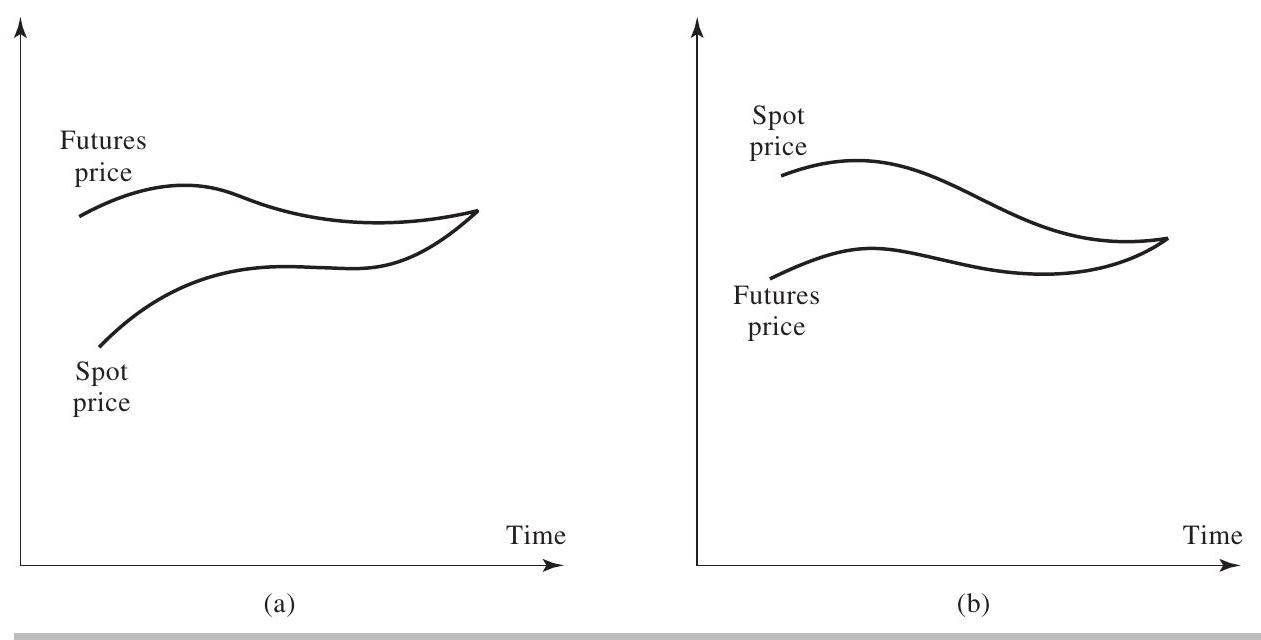
\includegraphics[width=\linewidth]{ead832f5-1069-4974-84bd-4a1adcf0b304-051_640_1261_384_361.jpg}
\caption{Convergence links the futures price to the spot price near delivery.}
\end{marginfigure}

The intuition is arbitrage. Suppose at delivery the futures price were above the
spot price. A trader could buy the asset in the spot market and deliver it into
the futures contract at the higher futures price. Suppose instead the futures
price were below the spot price. A trader who needs the asset could obtain it
through the futures contract more cheaply than in the spot market. Competitive
trading pressure closes the gap.

\begin{boxD}
\textbf{Convergence principle.} Delivery is rare in many futures markets, but
the possibility of delivery is what anchors the futures price to the spot price.
Without a credible settlement mechanism, a futures price could drift away from
the underlying cash market.
\end{boxD}

\subsection{Margin Accounts and Daily Settlement}

Margin is not a down payment on the asset. It is collateral that protects the
clearing system against default.

Let one futures contract be for $Q$ units of the underlying. Let $\Ft$ denote
the settlement futures price at the end of day $t$. For a long position in $N$
contracts, the daily gain or loss is
\[
    \pnl_t = NQ(\Ft-F_{t-1}).
\]
For a short position, the sign is reversed:
\[
    \pnl_t^{\mathrm{short}} = NQ(F_{t-1}-\Ft).
\]

If $M_t$ is the margin account balance after daily settlement and before any
margin call contribution, then
\[
    M_t = M_{t-1} + \pnl_t.
\]
If $M_t$ falls below the maintenance margin, the trader receives a margin call
and must restore the account to the initial margin level.

\begin{exmp}[Gold futures margin]
Suppose a trader is long two gold futures contracts. Each contract is for 100
ounces, so $NQ=200$ ounces. The initial futures price is USD 1,750 per ounce.
If the next settlement price is USD 1,741, the long position loses
\[
    200(1{,}741-1{,}750)=-\$1{,}800.
\]
The short side receives the same amount. Futures are zero-sum before transaction
costs, but the timing of cash flows differs because gains and losses are settled
daily.
\end{exmp}

\begin{boxF}
\textbf{Why daily settlement matters.} A forward contract accumulates gains and
losses until maturity. A futures contract realizes gains and losses every day.
This reduces counterparty credit risk, but it creates liquidity risk: a trader
can be economically right in the long run and still fail because margin calls
arrive before convergence.
\end{boxF}

\section{Options}

\subsection{Rights, Obligations, and Payoffs}

A call option gives the holder the right, but not the obligation, to buy the
underlying asset for strike price $\K$. A put option gives the holder the right,
but not the obligation, to sell the underlying asset for $\K$.

\begin{defN}[Option payoffs]
For a European option expiring at $T$,
\[
    \text{Call payoff} = \max(\St-\K,0)=(\St-\K)^+,
\]
and
\[
    \text{Put payoff} = \max(\K-\St,0)=(\K-\St)^+.
\]
\end{defN}

The option buyer has a right. The option seller, or writer, has an obligation.
This asymmetry is why the buyer pays an upfront premium.

If a call premium is $c_0$, the buyer's profit at maturity is
\[
    (\St-\K)^+ - c_0 e^{rT}
\]
when we account for the opportunity cost of the premium. If we ignore financing
over a short horizon, the common profit approximation is $(\St-\K)^+-c_0$.

\begin{marginfigure}
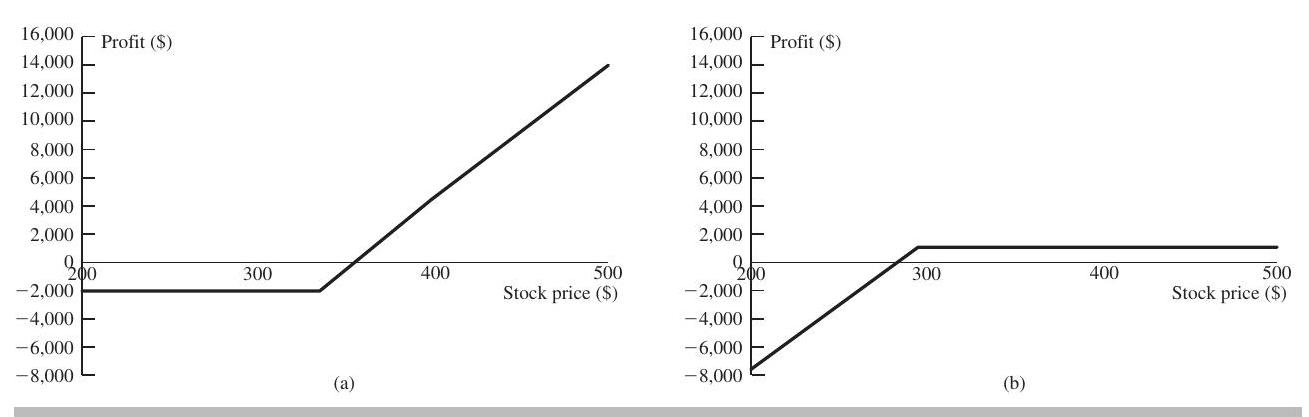
\includegraphics[width=\linewidth]{ead832f5-1069-4974-84bd-4a1adcf0b304-033_417_1309_425_361.jpg}
\caption{Option profits differ from payoffs because the option premium must be
paid upfront.}
\end{marginfigure}

\subsection{European and American Exercise}

A European option can be exercised only at maturity. An American option can be
exercised at any time up to maturity. The labels do not refer to geography.

American exercise rights are valuable because they give the holder more choices.
For a given underlying, strike, and maturity, an American option is worth at
least as much as the corresponding European option:
\[
    C_{\mathrm{American}} \geq C_{\mathrm{European}}, \qquad
    P_{\mathrm{American}} \geq P_{\mathrm{European}}.
\]
The inequality can be strict when early exercise has value.

\section{Hedgers, Speculators, and Arbitrageurs}

\subsection{Hedgers}

A hedger uses derivatives to reduce an existing exposure. The exposure exists
before the derivative trade. For example, an airline worried about jet fuel
prices may use energy derivatives. An exporter worried about foreign currency
receipts may use FX forwards. A fund manager worried about market declines may
use index futures or put options.

\begin{marginfigure}
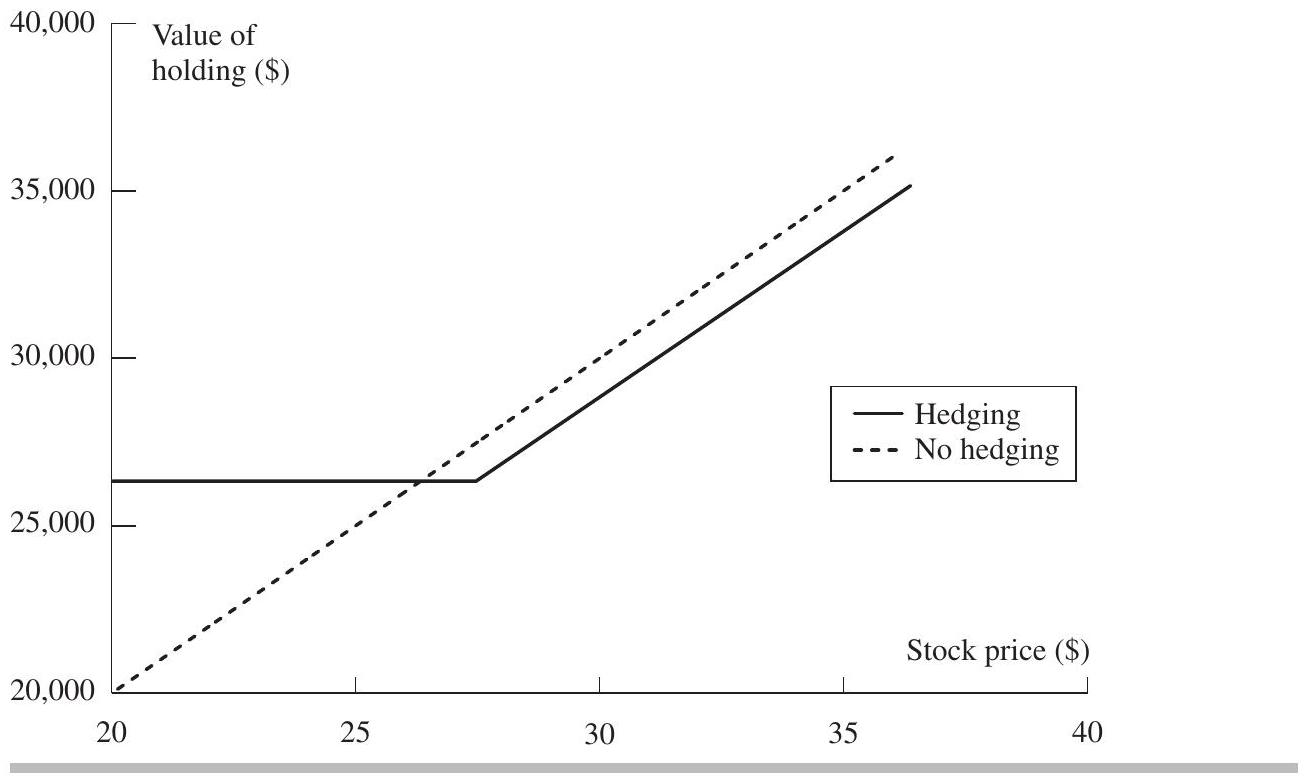
\includegraphics[width=\linewidth]{ead832f5-1069-4974-84bd-4a1adcf0b304-035_782_1309_1527_365.jpg}
\caption{A hedge reduces downside exposure but may also give up upside.}
\end{marginfigure}

The key question is not whether the derivative makes money. The key question is
whether the combined position has the desired risk profile. A hedge can lose
money and still be successful if the underlying exposure gains enough to offset
it.

\subsection{Speculators}

A speculator uses derivatives to take a view on the direction or volatility of a
market variable. Derivatives make speculation capital-efficient because the
initial cash outlay can be small relative to the notional exposure.

This is also the danger. Leverage magnifies both gains and losses. A futures
position may require only margin rather than full payment for the underlying,
but the economic exposure is to the full contract size.

\begin{marginfigure}
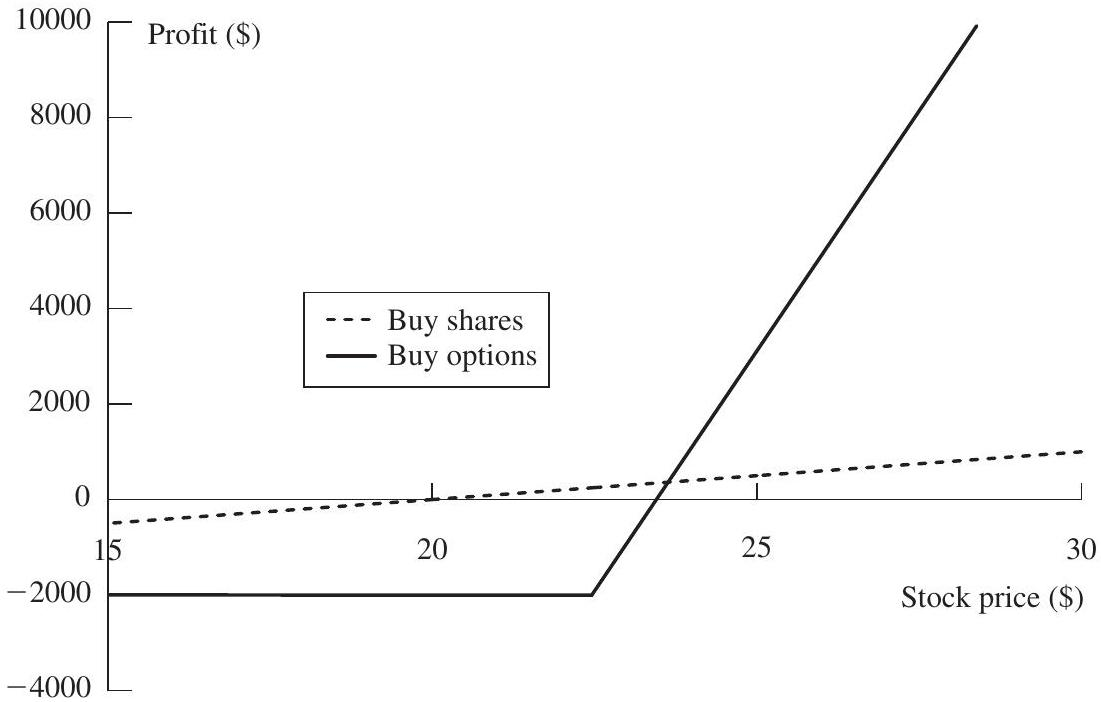
\includegraphics[width=\linewidth]{ead832f5-1069-4974-84bd-4a1adcf0b304-038_702_1101_398_458.jpg}
\caption{Leveraged derivative positions can create very different profit
profiles from direct investment in the underlying asset.}
\end{marginfigure}

\subsection{Arbitrageurs}

An arbitrageur tries to lock in a riskless profit by taking offsetting positions.
In theory, arbitrage should require no net investment, have no risk of loss, and
have a positive probability of profit. In practice, many trades called
``arbitrage'' are convergence trades: they are designed to profit when prices
move back toward a theoretical relationship, but they can lose money before that
happens.

\begin{boxF}
\textbf{Terminology warning.} True arbitrage is nearly riskless and self-financing.
Convergence trading is risky. It can fail because of funding constraints,
margin calls, crowded positions, model error, or liquidity shocks.
\end{boxF}

\section{Risk Lessons from Derivatives Mishaps}

Chapter 37 is useful at the start of the course because it prevents a common
mistake: treating derivatives as only equations. The equations matter, but the
institutions and controls matter too.

\subsection{A Taxonomy of Failure}

Large derivatives losses usually involve several failures at once:
\begin{enumerate}
    \item \textbf{Market risk.} The underlying market moves against the position.
    \item \textbf{Leverage.} The position is too large relative to capital.
    \item \textbf{Liquidity risk.} The trader cannot exit or fund the position
    when needed.
    \item \textbf{Model risk.} Prices, hedge ratios, or risk measures are wrong.
    \item \textbf{Operational risk.} Confirmations, settlement, booking, or
    reporting fail.
    \item \textbf{Governance failure.} Risk limits exist but are ignored,
    misunderstood, or overridden.
    \item \textbf{Incentive failure.} Traders or managers benefit from upside
    while losses are borne by the institution, clients, or taxpayers.
\end{enumerate}

\subsection{Risk Limits}

A risk limit is useful only if it is specific, measured, monitored, and enforced.
Examples include notional limits, value-at-risk limits, stress-loss limits,
Greek limits, stop-loss limits, maturity limits, counterparty limits, and
liquidity limits.

\begin{boxD}
\textbf{Good risk limit design.} A limit should answer four questions:
What exposure is being limited? How is it measured? Who sees the breach? What
happens when the breach occurs?
\end{boxD}

\subsection{Front, Middle, and Back Office}

Financial institutions separate trading activity into three functions.
\begin{description}
    \item[Front office] Initiates trades and manages client relationships or
    trading books.
    \item[Middle office] Measures risk, validates prices, monitors limits, and
    challenges assumptions.
    \item[Back office] Confirms trades, settles cash flows, maintains records,
    and reconciles positions.
\end{description}

The separation is not bureaucracy for its own sake. A trader who can both take
risk and control the reporting of that risk has too much unchecked authority.

\subsection{Model Risk}

A model is a simplified map of reality. In this course we will build models that
are extremely useful: no-arbitrage pricing, binomial trees, Black--Scholes--
Merton, Greeks, and volatility models. But the usefulness of a model does not
make it true.

Model risk appears when:
\begin{itemize}
    \item the wrong model is used for the product;
    \item parameters are estimated poorly;
    \item liquidity or transaction costs are ignored;
    \item correlations change in stress periods;
    \item the model is used outside the range where it was tested;
    \item users do not understand what the model assumes.
\end{itemize}

\begin{boxF}
\textbf{Rule for the course.} We will derive formulas carefully, but every
formula must be accompanied by its assumptions. A pricing formula without its
assumptions is not knowledge; it is a recipe for misuse.
\end{boxF}

\section{Lecture 1 Mathematical Toolkit}

\subsection{Positive Part Notation}

For any real number $x$,
\[
    x^+ = \max(x,0).
\]
Thus the call payoff is $(S_T-K)^+$ and the put payoff is $(K-S_T)^+$.

\subsection{Linear Versus Convex Payoffs}

A forward payoff is linear in $S_T$:
\[
    g(S_T)=S_T-K.
\]
Its slope with respect to $S_T$ is one everywhere:
\[
    \frac{d g}{dS_T}=1.
\]

A call payoff is convex:
\[
    g(S_T)=(S_T-K)^+.
\]
Ignoring the kink at $S_T=K$, its slope is
\[
    \frac{d g}{dS_T}
    =
    \begin{cases}
    0, & S_T<K,\\
    1, & S_T>K.
    \end{cases}
\]
This kink is the source of much of option-pricing theory. Linear exposures can
often be hedged with fixed quantities. Nonlinear exposures require dynamic
hedging or option-pricing models.

\subsection{Simple Arbitrage Logic}

Most no-arbitrage arguments follow the same structure:
\begin{enumerate}
    \item Identify two strategies with the same future payoff.
    \item Compute their current costs.
    \item If the costs differ, buy the cheaper strategy and sell the expensive
    strategy.
    \item The price discrepancy cannot persist in a competitive market.
\end{enumerate}

In the forward-price derivation, the two strategies are:
\[
    \text{buy stock now and finance it}
    \quad \text{versus} \quad
    \text{enter forward to buy later}.
\]
Both deliver ownership of one share at time $T$. Therefore their costs must be
consistent.

\section{Worked Problems}

\begin{exmp}[Forward hedge payoff]
A firm will receive EUR 10 million in three months. It enters a short forward
contract at USD 1.0800 per EUR. At maturity, the spot exchange rate is USD
1.0350 per EUR.

The short forward payoff per euro is
\[
    K-S_T = 1.0800-1.0350 = 0.0450.
\]
For EUR 10 million, the derivative payoff is
\[
    0.0450 \times 10{,}000{,}000 = \$450{,}000.
\]
The receivable itself is worth fewer dollars when the euro falls. The forward
gain offsets that loss. The firm has locked in
\[
    1.0800 \times 10{,}000{,}000 = \$10.8\text{ million}.
\]
\end{exmp}

\begin{exmp}[No-arbitrage forward price]
A non-dividend-paying stock has $S_0=50$. The continuously compounded risk-free
rate is $r=4\%$ and $T=0.5$ years. The no-arbitrage forward price is
\[
    F_0 = 50e^{0.04\times 0.5}
    = 50e^{0.02}
    \approx 51.01.
\]
If the six-month forward price were 53, the cash-and-carry arbitrage would be:
borrow 50, buy the stock, and short the forward. The locked-in terminal profit
would be
\[
    53-50e^{0.02} \approx 1.99.
\]
\end{exmp}

\begin{exmp}[Margin account]
A trader is long one futures contract on 1,000 units. The settlement price falls
from 82.40 to 81.75. The daily futures P\&L is
\[
    1 \times 1{,}000(81.75-82.40)=-650.
\]
The long loses 650 and the short gains 650. If the long's margin account was
2,200 before settlement, it becomes 1,550 after settlement. If maintenance
margin is 1,600, a margin call is triggered.
\end{exmp}

\section{Checklist for Students}

After this lecture you should be able to:
\begin{itemize}
    \item define derivative, underlying, payoff, profit, value, notional, and
    market value;
    \item distinguish exchange-traded and OTC derivatives;
    \item explain the role of clearing houses, CCPs, margin, and collateral;
    \item write long and short forward payoffs;
    \item derive $F_0=S_0e^{rT}$ for a non-dividend-paying asset;
    \item explain why futures prices converge to spot prices near delivery;
    \item compute daily futures gains and losses from settlement prices;
    \item write call and put payoffs using positive-part notation;
    \item distinguish hedging, speculation, true arbitrage, and convergence
    trading;
    \item identify common causes of derivatives losses.
\end{itemize}

\section{Practice Questions}

\begin{enumerate}
    \item A long forward has delivery price $K=120$. Draw and label the payoff
    diagram. What is the payoff if $S_T=95$, $120$, and $138$?
    \item A stock has price $S_0=80$, pays no dividends, and the continuously
    compounded risk-free rate is 3\%. Compute the one-year no-arbitrage forward
    price. Describe the arbitrage if the quoted forward price is 85.
    \item A trader is short three futures contracts. Each contract is for 5,000
    units. The settlement price changes from 4.62 to 4.55. Compute the daily
    P\&L.
    \item Explain why margin is not the same as the price of a futures contract.
    \item A European call has strike $K=50$ and premium $c_0=4$. Compute the
    payoff and approximate profit at maturity for $S_T=42$, $50$, and $63$,
    ignoring financing of the premium.
    \item Give one example of a hedge, one example of speculation, and one
    example of a trade often called arbitrage that is actually convergence
    trading.
    \item Pick one derivatives mishap discussed in class. Identify at least
    three distinct risk-management failures involved.
\end{enumerate}

\end{document}
